\chapter{Market and Stakeholder Analysis}
\setlength{\parindent}{15pt}
\label{ch:mark_stak_anal}

%Total chapter max 4 pages
In this chapter, both the market and stakeholder analyses are presented. The size of the market and competitors are identified in \autoref{ec:mark_anal}. Then all stakeholders of the project are listed and their relevance is explained in \autoref{sec:stak_anal}.

\section{Market Analysis}
\label{ec:mark_anal}


\begin{comment}
- 3 pages in baseline report
- pretty general
- structure
    - market definition
    - current + expected market size
    - competition analysis
    - customer analysis
    - conclusion

This report:
- general overview + size estimation
- outline competitors
- maybe give expectations
- 1-2 pages since stakeholders also need to be included

- try do give an estimation of the AMOUNT of UAVs that we can sell for the cost analysis


Already determined/stated in baseline report:
- UAV part of general aviation sector, footnote http://www.iaopa.org/what-is-general-aviation/ 1-5-17
- Defined market: The subsets of both the general aviation market and military market comprising UAVs and helicopters used specifically for autonomous monitoring and transport missions.
- Very hard to quantify market size and potential. Estimation set at --
 The entire UAV market is estimated to be worthUS Dollar (USD) 13.22 billion and is expected to double in value over the next five years.
 REF 4http://www.marketsandmarkets.com/Market-Reports/unmanned-aerial-vehicles-uav-market-662.html?gclid=Cj0KEQjwuZvIBRD-8Z6B2M2Sy68BEiQAtjYS3D4gmcrdpSawOfsX6w4PIEX91fD4cpe7P7stNjVpG9IaAu3c8P8HAQ,Last accessed 01-05-2017
- competition analysis
\end{comment}





In this section, a market analysis relevant to the Hybrid UAV is presented. First, the market is defined, and its current size and expected growth are estimated. Then an analysis of the competition is made. Finally, a customer analysis is made, which is partly based on the stakeholders as discussed in \autoref{sec:stak_anal}.




\subsection{Current and Future Market}
\label{sec:curr_futu_mark}

In the baseline report, the market was already analysed \cite{baseline}. The Hybrid UAV will be part of the general aviation  sector\footnote{\url{http://www.iaopa.org/what-is-general-aviation/}, Accessed on 01-05-2017}. Its market can be defined as:

\begin{quote}
\begin{itshape}
The subsets of both the general aviation market and military market comprising UAVs and helicopters used specifically for autonomous monitoring and transport missions.
\end{itshape}
\end{quote}

During the previous analysis, it was also determined that quantifying the market size is extremely difficult. The current estimation is that the entire UAV market is worth United States Dollar (USD) 13.22 billion\footnote{\url{http://www.marketsandmarkets.com/Market-Reports/unmanned-aerial-vehicles-uav-market-662.html?gclid=Cj0KEQjwuZvIBRD-8Z6B2M2Sy68BEiQAtjYS3D4gmcrdpSawOfsX6w4PIEX91fD4cpe7P7stNjVpG9IaAu3c8P8HAQ}, Accessed on 01-05-2017} (12.11 billion EUR), while the market opportunity between now and 2020 is estimated at USD 100 billion\footnotemark (92 billion EUR\footnotemark). The relevant part of the market for the Hybrid UAV that is being designed, is estimated at USD 13 billion (12 billion EUR) in this period\footnotemark. Shese values should mostly be considered for their order of magnitude, since the exact market size is nearly impossible to grasp. %The market share that can be used to sell the Winged Quadcopter is expected 

\footnotetext{Exchange rate 1 USD = 0.92 EUR, 26-06-2017}
\footnotetext{\label{ft:market_value}\url{http://www.goldmansachs.com/our-thinking/technology-driving-innovation/drones/}, Accessed 22-06-2017}
\footnotetext{See \autoref{ft:market_value}.}


\nomenclature[A]{USD}{United States Dollar}



\subsection{Competition Analysis}
Since the market is growing, it is expected to provide enough business opportunities. Therefore, an analysis of the competition is made, which is the most important information on the market during the design process. When the design is too similar to a product that is already on the market, chances of success are smaller. In the baseline report, not only UAVs, but also helicopters were included in this analysis. A choice was made to leave helicopters out of the analysis in this report, since even though they are used a lot for the same missions, most customers will specifically look for a UAV. Also UAVs weighing over 25 kg were not considered because of EASA regulations; this ruled out a lot of companies and models, such as Textron and most of Latitudes models. The largest difference between this Hybrid UAVs main market orientation and that of the competition is that other UAVs are much more mission specific.%so our thing is more versatile
\nomenclature{EASA}{European Aviation Safety Agency}

\begin{table}[hbt]
    \centering
    \caption{List of Competitors}
    \label{tab:list_comp}
    \begin{tabularx}{\textwidth}{>{\small}p{.126\textwidth} L  L >{\small}p{.12\textwidth} }
    \toprule
    \textbf{Company, concept}     & \textbf{Unique selling points and benefits} & \textbf{Commonalities and outperformed aspects}  &\textbf{Price estimate} 
    \\ \midrule
    Latitude, HQ-40\footnotemark    & Cooperate with Arcturus and Textron by using their airframes, and also enable the use of other airframes in combination with their quadrotor technology. Gas powered. & Hybrid quadrotor layout. Most competing concept has five hour endurance and 2.5 kg payload capacity. & USD 40,000\footnotemark
    \\ \hdashline
    Arcturus, Jump-15\footnotemark & Endurance 6+ hours, catapult launch. & Hybrid quadrotor layout. Maximum speed 100 km/h, fuel injection engine. & Unknown
    \\ \hdashline
    Avy         & Prandtl box layout. 400 km range. & Maximum speed 200 km/h, 10 kg payload, fully electric\footnotemark. & EUR 30,000 - 60,000\footnotemark
    \\ \hdashline
    Atmos       & Tailsitter concept. MTOW estimated at 5,5 kg\footnotemark, fully electric. & Meant for mapping missions, such as precision agriculture. Mapping range 1 square km, endurance 30 minutes. & Estimated at EUR 30,000
    \\ \hdashline
    Carbonix, Volanti\footnotemark    & Multiple modular options. Endurance 1.5 h when operated fully electric.& Hybrid twin- or quadrotor layout. Optimal loiter speed 65 km/h. Payload bay ca. 0.4x0.2x0.1 m, capacity 6 kg. & Estimated at USD 114,000\footnotemark
    \\ \hdashline
    Sky-watch, Cumulus and Heidrun\footnotemark   & Deep stall landing, hand launched.  & Up to 600 g payload capacity, 25 km range or 40 square km coverage in monitoring, top speed 100 km/h. & Unknown
    \\ \bottomrule
    \end{tabularx}
\end{table}
\nomenclature{MTOW}{Maximum Take Off Weight}

\addtocounter{footnote}{-9}
\stepcounter{footnote}\footnotetext{\url{https://latitudeengineering.com/products/hq/}, Accessed 08-06-2017}
\stepcounter{footnote}\footnotetext{\url{http://www.popularmechanics.com/flight/drones/a9351/this-unmanned-plane-can-land-on-a-helo-pad-15812116/}, Accessed 08-06-2017}
\stepcounter{footnote}\footnotetext{\url{https://www.uav-africa.com/.../11_arcturus-jump-spec-sheet.pdf}, Accessed 08-06-2017}
\stepcounter{footnote}\footnotetext{\url{www.avy.eu}, Accessed 08-06-2017}
\stepcounter{footnote}\footnotetext{Private contact with Avy}
\stepcounter{footnote}\footnotetext{Private contact with Atmos}
\stepcounter{footnote}\footnotetext{\url{http://carbonix.com.au/wp-content/uploads/2017/02/17-02-22-Carbonix-VTOL-Hybrid-UAV-Information-Brochure.pdf}, Accessed 08-06-2017}
\stepcounter{footnote}\footnotetext{\url{http://newatlas.com/carbonix-volanti-vtol-fixed-wing-industrial-uav/48253/}, Accessed 08-06-2017}
\stepcounter{footnote}\footnotetext{\url{http://sky-watch.com/products/}, Accessed 08-06-2017}





\subsection{Customer Analysis}
There exist different types of potential customers. These are defined by the mission types the Hybrid UAV can perform, and have some overlap with the stakeholders. Some customer groups are: governmental organisations, non-governmental non-profit organisations (charities), farmers, logistics companies, internet retailers, offshore companies, infrastructure companies, and hospitals. 


Both opportunities and difficulties arise because of this large range of potential customers. A lot of UAVs can be sold, yet promoting the product in so many different sectors is time consuming. Also, the versatile nature of the Winged Quadcopter design might not be as attractive as a UAV solely designed for the customers intended purpose.


Aspects regarding the potential sales of the Hybrid UAV combined with the estimated market size from \autoref{sec:curr_futu_mark}, the amount of UAVs team 14 will sell can be estimated. The estimated sales price is 60,000 euros (EUR). When team 14 is able to take 0.25\% of the civil UAV market, that would mean that the team could sell for EUR 32 million on drones\footnotemark. That means around 500 Hybrid UAVs can be sold.
\nomenclature[A]{EUR}{Euro}


\footnotetext{Exchange rate USD 1 = EUR 0.92, 23-06-2017}




\section{Stakeholder Identification and Analysis}
\label{sec:stak_anal}


Stakeholders of a project are actors, namely persons or organisations who have a vested interest in the success of the project \cite{gotstake}. They are individuals or groups who are affected by or who can exert influence on the project's outcome. The stakeholders can range from organisations who govern policy of the project, to citizens who may benefit or be disadvantaged depending on the outcome of the project. The success of a project in project management terms is partially defined by stakeholder satisfaction and therefore, in order to successfully execute the project, it is crucial to conduct a stakeholder analysis.

In order to conduct a stakeholder analysis, the relevant stakeholders must first be identified. Once the stakeholders are identified the analysis can be conducted which would include investigating the ability of each stakeholder to affect the project as well as their interest in the project. Each stakeholder will be presented followed by both an individual analysis and a potential management strategy. Finally a graphical representation of the analysis will be presented.


\subsection{Identification and Analysis}
In this section the direct stakeholders will be identified and analysed based on a few key aspects. Each stakeholders' knowledge of the project and interest in the project will be examined as well, to identify whether they are for or against the project. Each stakeholders' power (ability) to affect the project will be assessed as well as whether potential alliances with other stakeholders could be in store. Each stakeholder will be rated from 1 to 4 on both power and interest, 1 being given to stakeholders who have little power or interest, and 4 to stakeholders that have significant power over or interest in the project. The ratings will be presented as \textbf{(\textit{interest, power})}.

\paragraph{A. Avy}
Avy has laid out the primary requirements of the design of the Hybrid UAV and therefore, by definition, has significant power over the outcome of the project as well as substantial knowledge about the project. Avy might adopt the findings of the project, however that is at their own discretion and therefore their interest in the project is moderate. Rating \textbf{(\textit{2, 3})} 

\paragraph{B. EASA}
EASA is responsible for regulating European Aviation and therefore, in order to get certification to operate the Hybrid UAV developed throughout this project, EASA airworthiness regulations must be met. The project cannot be a success without meeting these requirements and therefore EASA has substantial power over the project. Rating \textbf{(\textit{1, 4})} 

\paragraph{C. General Public}
Ultimately the goal of the project is to develop a product that serves the general public and therefore the public in theory has a high interest in the project. However, it is most likely that the vast majority of the public will not have much knowledge about the project and it's goals. Since the Hybrid UAV is to be operated in the public domain, there needs to be transparency as pertains to the development and operation of the UAV. There will be a subset of the general public who will be against the project as they might see the product as being potentially harmful to their quality of life (privacy and noise pollution). The wishes of the public must be considered and therefore the public's ability to affect the project is moderate. Rating \textbf{(\textit{2, 2})} 

\paragraph{D. National Fire Department}
National fire departments are potential customers as fire departments are generally in charge of search and rescue efforts. Fire departments will therefore be in support of the successful execution of the project and will be interested in the capabilities of the Hybrid UAV. As potential operators of the UAV, input from the fire departments must be considered and therefore the fire departments exercise moderate power over the project. Rating \textbf{(\textit{3, 2})} 

\paragraph{E. Health Care Institutions}
As potential customers of a product aiming to decrease the transport time of emergency medical supplies and samples, health care institutions will be beneficiaries of the successful execution of the project. They will therefore be interested in the progress made throughout the development phase. Medical institutions will have substantial power over the design as the UAV must meet the stringent requirements on the conditions required for delicate transportation missions. Rating \textbf{(\textit{3, 2})} 

\paragraph{F. Infrastructure \& Asset Owners}
The Hybrid UAV will have the capabilities required for highly accurate surveillance. This makes it an attractive product for owners and operators of extensive infrastructure and expensive assets as monitoring costs can be drastically decreased. As the outcome of the project is simply a product that can be bought and configured for specific missions, infrastructure and asset owners do not have significant power or leverage over the execution of the project. Rating \textbf{(\textit{2, 3})} 

\paragraph{G. Logistics Companies}
As potential customers, logistics companies will be interested in the capabilities of the Hybrid UAV. They will be particularly interested in the relationship between range and payload. Ultimately, the logistics companies do not have substantial leverage over the project. However, as potential customers, whether or not their wishes are met dictates to some degree the success of the project. Rating \textbf{(\textit{2, 3})} 

\paragraph{H. Suppliers of Parts \& Services}
During the production phase of the project, various 'off the shelf' components as well as a number of services will be required to successfully produce the Hybrid UAV. The costs dictated by the suppliers have a substantial effect on the overall production costs of the UAV and therefore the suppliers have significant power over the project. Suppliers are not particularly interested in the project but rather in the business opportunity of supplying parts or services. Rating \textbf{(\textit{1, 3})} 

\paragraph{I. Air Traffic Control}
Air traffic control is responsible for regulating air traffic to ensure safety for all. Air traffic control needs to keep an overview of all air traffic in certain airspace regions and has the authority to stipulate what class of aircraft is allowed to be operated in what regions of airspace. For this reason, they, along with the EASA regulatory body, pose constraints on the outcome of the project and the types of missions that can be carried out. Air traffic control agencies have no particular interest in the project and are likely to be neither for or against the project. Rating \textbf{(\textit{1, 3})}

\paragraph{J. Sponsors}
Sponsors give something of value to the project (money, expertise, a service, access to facilities, etc.) and in return receive good publicity. Because of providing something of value to the project (usually vital to the success of the project), sponsors have significant power over the project and are particularly interested in the successful execution of the project. Rating \textbf{(\textit{4, 3})} 

\subsection{Summary of Stakeholder Analysis}
Having analysed the direct stakeholders and rated each on the basis of interest and power, each stakeholder can be mapped to a specific management strategy as shown in \autoref{fig:stake_map}. These management strategies are:

\indent \textbf{Manage Closely} which would entail constantly keeping the stakeholder up to date with progress. This can be done with, for example, status meetings. Stakeholders in this category are in the top right of the figure.\\
\indent \textbf{Keep Satisfied} through close conversation with the stakeholder about goals and wishes along with keeping the stakeholder up to date with progress. Stakeholders in this category are in the top left of the figure.\\
\indent \textbf{Keep informed} about the general progress. This might be done in-person or through the media. Stakeholders in this category are in the bottom right of the figure.\\
\indent \textbf{Monitor} by keeping the stakeholder in contact. Stakeholders in this category are in the bottom left of the figure.


\begin{figure}[h]
    \centering
    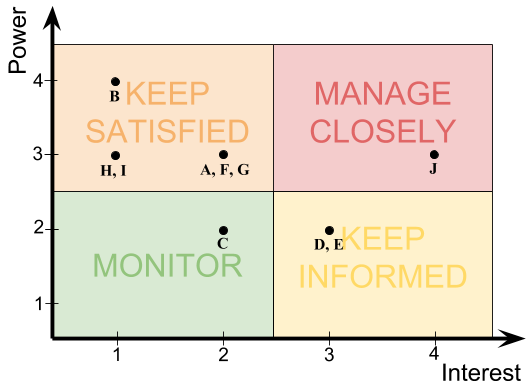
\includegraphics[scale=0.5]{MarketStakeholderAnalysis/Figures/Stakeholder_mapping}
    \caption{Mapping of Stakeholders Based on Interest and Power}
    \label{fig:stake_map}
\end{figure}